\documentclass[12pt]{article}

\usepackage{sbc-template}
\usepackage{graphicx,url}
\usepackage[brazil]{babel}   
\usepackage[utf8]{inputenc}
\usepackage{enumitem}
\usepackage{placeins}

\hyphenation{english terms to not hyphenize various non repeatable words here something like long word Portuguese}
     
\sloppy

\title{Análise de Eficiência Energética e Desempenho da Paralelização do Processamento de Imagens com Filtros Convolucionais}

\author{Enzo de Almeida Belfort Rizzi Di Chiara\inst{1}, Luiza de Souza Ferreira\inst{1}, Natália Vitória\\Amaral do Val\inst{1}, Vinícius Augusto Landim Andrade\inst{1}, Viviane Flor Park\inst{1} 
}


\address{Instituto de Ciência e Tecnologia -- Universidade Federal de São Paulo (UNIFESP) \\ São José dos Campos -- SP -- Brasil
\email{\parbox{\textwidth}{\centering\{belfort.enzo, souza.luiza, amaral.natalia, vinicius.landim, \\ viviane.park\}@unifesp.br}}
}

\begin{document} 

\maketitle

\begin{abstract}
  This article describes the implementation of a parallelized version of a convolutional filter algorithm and the corresponding analysis of its energy efficiency and performance. The algorithm is parallelized in two different ways -- using the OpenMP library and the CUDA platform -- and each version is tested with a set of images of varying dimensions. The results of the parallel implementations are compared against the sequential version of the algorithm and against each other in terms of execution time, speedup, and energy efficiency.
\end{abstract}
     
\begin{resumo} 
  Este artigo descreve a implementação de uma versão paralelizada de um algoritmo de filtro convolucional e sua respectiva análise de eficiência energética e desempenho. A paralelização do algortimo é feita de duas maneiras diferentes, com a biblioteca OpenMP e a plataforma CUDA, e cada versão é testada com um conjunto de imagens com diferentes dimensões. Os resultados das implementações paralelas são comparados com a versão sequencial do algoritmo e entre si em termos de tempo de execução, speedup e eficiência energética.
\end{resumo}


\section{Introdução}

% apresentação do problema, contextualização e objetivos

\section{Fundamentação Teórica e Trabalhos Relacionados}

% filtros convolucionais
% paralelização com OpenMP / CUDA
% métricas de desempenho
% apresentação de ~2(?) trabalhos relacionados

\section{Metodologia e Implementação}

% como foi implementada a paralelização
% apresentar hardware usado e outras bibliotecas utilizadas
% casos de teste

\section{Resultados e Discussão}

% análise das métricas de desempenho coletadas

\section{Conclusão}

% resumo dos principais resultados
% 

% ---------------------------------------------------
% EXEMPLOS DE FIGURAS E TABELAS
% ---------------------------------------------------
% \begin{figure}[ht]
% \centering
% 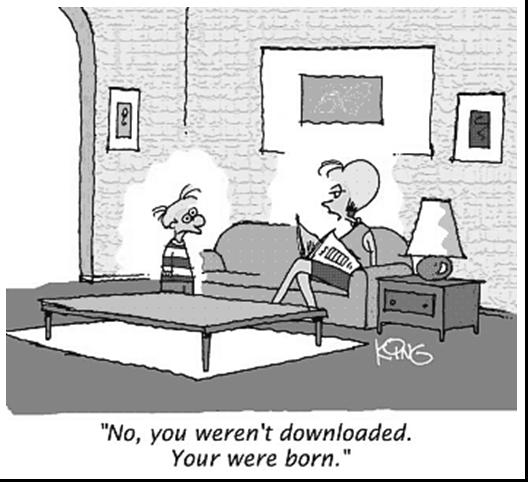
\includegraphics[width=.5\textwidth]{fig1.jpg}
% \caption{A typical figure}
% \label{fig:exampleFig1}
% \end{figure}

% \begin{figure}[ht]
% \centering
% 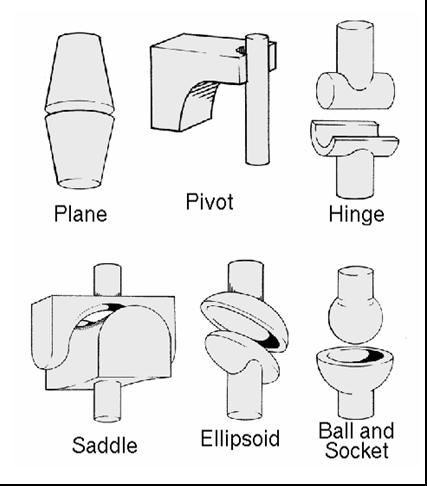
\includegraphics[width=.3\textwidth]{fig2.jpg}
% \caption{This figure is an example of a figure caption taking more than one
%   line and justified considering margins.}
% \label{fig:exampleFig2}
% \end{figure}

% \begin{table}[ht]
% \centering
% \caption{Variables to be considered on the evaluation of interaction
%   techniques}
% \label{tab:exTable1}
% 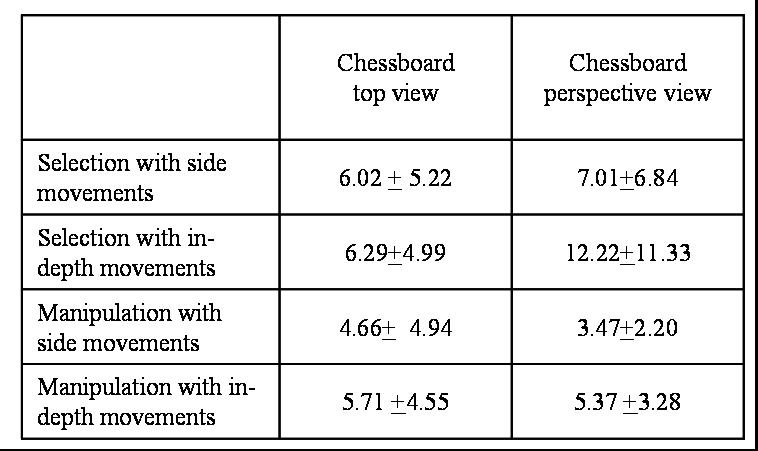
\includegraphics[width=.7\textwidth]{table.jpg}
% \end{table}

\bibliographystyle{sbc}
\bibliography{sbc-template}

\end{document}
